\documentclass[11pt]{article}\usepackage[]{graphicx}\usepackage[]{color}

\usepackage{alltt}
\usepackage[margin=1in]{geometry}   % set up margins
\usepackage[T1]{fontenc}
\usepackage{xcolor}                 % allows color
\usepackage{enumerate}              % fancy enumerate
\usepackage{amsmath}
\usepackage{amsthm}
\usepackage{amssymb}              % used for \eqref{} in this document
\usepackage{verbatim}               % useful for \begin{comment} and \end{comment}
\usepackage{eurosym}                % used for euro symbol
\usepackage{tabularx}
\usepackage{caption} 
\usepackage{graphicx}
\usepackage{subcaption}
\usepackage{color, colortbl}
\usepackage{indentfirst}
\usepackage{hyperref}
\usepackage{booktabs}
\usepackage{tabularx}
\usepackage{mathrsfs}
\usepackage{dsfont}
\usepackage{sgamevar}
\usepackage{sgame}
\usepackage{tikz}
\hypersetup{colorlinks, linkcolor=blue}
\usetikzlibrary{snakes}

\setlength\parindent{0pt}

\setlength\parindent{0pt}

\begin{document}
	
\title{\textbf{Where Does the ``Rule of 70'' Come From?} \\ \vspace{2 mm} {\large ECON 101}}
\author{David A. D\'iaz\footnote{Any mistakes in this document are my own. Not for circulation.}}
\date{\today}
\maketitle

You hopefully know from class that for a variable (say, real GDP) that grows at a constant rate $g$ every period, the approximate time it takes for that variable to double in size is 

\begin{equation}
\label{eq1}
T_2 \approx \frac{70}{g},
\end{equation}

where $g$ is expressed in percent form. This is the so-called ``Rule of 70.'' 
\\

For example, if real GDP grows at 5\% each year in country $A$, then country $A$'s real GDP would double in approximately $70/5 = 14$ years.
\\

Here, we will see where this ``rule'' comes from.

\subsection*{Compound Growth}

To make life easy, let's focus on the growth of real GDP, $Y$. We start at time $t=0$ with some stock of real GDP, $Y_0$. Real GDP grows at rate $g$ each period and we want to know how long it takes real GDP to double, i.e., reach a real GDP level of $2\times Y_0$. Let's label this time $T_2$.
\\

If real GDP is $Y_0$ in period 0, then in period 1 it will be $Y_1 = Y_0(1+g)$, where here $g$ is expressed in decimal form (e.g., $g=.05$). In period 2, real GDP is $Y_2 = Y_1(1+g) = Y_0(1+g)^2$. Continuing this, real GDP in any period $t$ is given by 

\begin{equation}
\label{eq2}
Y_t = Y_0(1+g)^t. 
\end{equation}

Here is a pretty timeline to help see what's going on:
\\

\begin{center}
	
 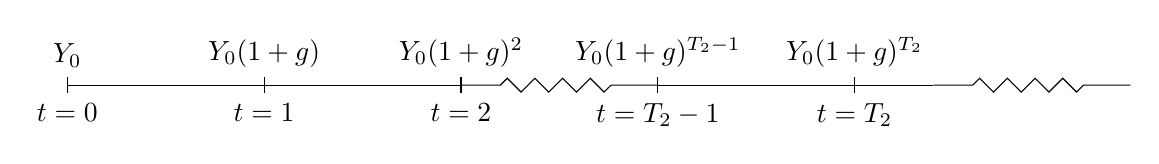
\begin{tikzpicture}[snake=zigzag, line before snake = 5mm, line after snake = 5mm]
 % draw horizontal line   
 \draw (0,0) -- (5,0);
 \draw[snake] (5,0) -- (7.5,0);
 \draw (7.5,0) -- (11,0);
 \draw[snake] (11,0) -- (13.5,0);
 
 % draw vertical lines
 \foreach \x in {0,2.5,5,7.5,10}
 \draw (\x cm,3pt) -- (\x cm,-3pt);
 
 % draw nodes
 \draw (0,0) node[below=3pt] {$ t=0 $} node[above=3pt] {$ Y_0  $};
 \draw (2.5,0) node[below=3pt] {$ t=1 $} node[above=3pt] {$ Y_0(1+g) $};
 \draw (5,0) node[below=3pt] {$ t=2 $} node[above=3pt] {$ Y_0(1+g)^2 $};
 \draw (7.5,0) node[below=3pt] {$ t=T_2-1 $} node[above=3pt] {$ Y_0(1+g)^{T_2-1} $};
 \draw (10,0) node[below=3pt] {$ t=T_2 $} node[above=3pt] {$ Y_0(1+g)^{T_2} $};
 \end{tikzpicture}

\end{center}

Real GDP at $T_2$ is $Y_{T_2} = Y_0(1+g)^{T_2}$. But if real GDP has doubled at $T_2$, then $Y_{T_2} = 2Y_0$. Equating the two expressions, we have

\begin{equation}
\label{eq3}
2Y_0 = Y_0(1+g)^{T_2}.
\end{equation}

\newpage

\subsection*{Teeny Bit of Algebra (and Calc)}

From Equation (\ref{eq3}), we can solve for $T_2$:

\[2Y_0 = Y_0(1+g)^{T_2} \Rightarrow 2 = (1+g)^{T_2} \Rightarrow \ln(2) = T_2 \times \ln(1+g)\Rightarrow T_2 = \frac{\ln(2)}{\ln(1+g)}.\]

Woo, we have the formula for the \textit{actual} doubling time!
\\

Thus, the true doubling time for country $A$'s real GDP is $\ln(2)/\ln(1.05) = 14.207$ years. The approximation is pretty close, eh?
\\

Now, notice that $\ln(2) \approx .693$. To simplify further, let's go with $\ln(2) \approx .70$. 
\\

A linear approximation of $\ln(1+g)$ gives us that $\ln(1+g) \approx g$ for $g$ close to 0.\footnote{This comes from a Taylor series expansion of $\ln(1+x)$ around $x=0$. Remember from calculus that a Taylor series of $f(x)$ around $x=a$ is given by $f(a) + \frac{f'(a)}{1!}\cdot(x-a) + \frac{f''(a)}{2!}\cdot(x-a)^2 + \frac{f'''(a)}{3!}\cdot(x-a)^3 + \dots$. So, a linear approximation around $x=0$ is given by $f(x) \approx f(0) + \frac{f'(0)}{1!}\cdot x$. For $f(x) = \ln(1+x)$, we have $f(0) = \ln(1) =0$, $f'(x) = 1/(1+x)$, and $f'(0) = 1/(1+0) = 1$. Thus, $\ln(1+x) \approx x$.} 
\\

Putting those together, we have where our approximation for doubling times comes from: 


\[T_2 \approx \frac{.70}{\underbrace{g}_{\text{in decimal form}}} = \frac{.70}{g} \times \frac{100}{100} = \frac{70}{100g} = \frac{70}{\underbrace{g}_{\text{in percent form}}}.  \]

\subsection*{For You}
What is the true formula for the quadruple time, $T_4$, and the eight-fold time, $T_8$? What could be the ``Rule'' for each?
\vspace{3cm}


\color{black}
What is the quadrupling time expressed in terms of $T_2$ (i.e., write $T_4$ as a function of $T_2$)? The eight-fold time? \textbf{Hint:} A property of logs is that $\ln(x^a) = a\times \ln(x)$.




\end{document}